\documentclass[
	% -- opções da classe memoir --
	12pt,				% tamanho da fonte
	openright,			% capítulos começam em pág ímpar (insere página vazia caso preciso)
	%twoside,			% para impressão em recto e verso. Oposto a oneside
	oneside,      % para impressão direta das páginas. Oposto a twoside
	a4paper,			% tamanho do papel.
	% -- opções da classe abntex2 --
	%chapter=TITLE,		% títulos de capítulos convertidos em letras maiúsculas
	%section=TITLE,		% títulos de seções convertidos em letras maiúsculas
	%subsection=TITLE,	% títulos de subseções convertidos em letras maiúsculas
	%subsubsection=TITLE,% títulos de subsubseções convertidos em letras maiúsculas
	% -- opções do pacote babel --
	english,			% idioma adicional para hifenização
	french,				% idioma adicional para hifenização
	spanish,			% idioma adicional para hifenização
	brazil,				% o último idioma é o principal do documento
	]{abntex2}\usepackage[]{graphicx}\usepackage[table]{xcolor}
% maxwidth is the original width if it is less than linewidth
% otherwise use linewidth (to make sure the graphics do not exceed the margin)
\makeatletter
\def\maxwidth{ %
  \ifdim\Gin@nat@width>\linewidth
    \linewidth
  \else
    \Gin@nat@width
  \fi
}
\makeatother

\definecolor{fgcolor}{rgb}{0.345, 0.345, 0.345}
\newcommand{\hlnum}[1]{\textcolor[rgb]{0.686,0.059,0.569}{#1}}%
\newcommand{\hlstr}[1]{\textcolor[rgb]{0.192,0.494,0.8}{#1}}%
\newcommand{\hlcom}[1]{\textcolor[rgb]{0.678,0.584,0.686}{\textit{#1}}}%
\newcommand{\hlopt}[1]{\textcolor[rgb]{0,0,0}{#1}}%
\newcommand{\hlstd}[1]{\textcolor[rgb]{0.345,0.345,0.345}{#1}}%
\newcommand{\hlkwa}[1]{\textcolor[rgb]{0.161,0.373,0.58}{\textbf{#1}}}%
\newcommand{\hlkwb}[1]{\textcolor[rgb]{0.69,0.353,0.396}{#1}}%
\newcommand{\hlkwc}[1]{\textcolor[rgb]{0.333,0.667,0.333}{#1}}%
\newcommand{\hlkwd}[1]{\textcolor[rgb]{0.737,0.353,0.396}{\textbf{#1}}}%
\let\hlipl\hlkwb

\usepackage{framed}
\makeatletter
\newenvironment{kframe}{%
 \def\at@end@of@kframe{}%
 \ifinner\ifhmode%
  \def\at@end@of@kframe{\end{minipage}}%
  \begin{minipage}{\columnwidth}%
 \fi\fi%
 \def\FrameCommand##1{\hskip\@totalleftmargin \hskip-\fboxsep
 \colorbox{shadecolor}{##1}\hskip-\fboxsep
     % There is no \\@totalrightmargin, so:
     \hskip-\linewidth \hskip-\@totalleftmargin \hskip\columnwidth}%
 \MakeFramed {\advance\hsize-\width
   \@totalleftmargin\z@ \linewidth\hsize
   \@setminipage}}%
 {\par\unskip\endMakeFramed%
 \at@end@of@kframe}
\makeatother

\definecolor{shadecolor}{rgb}{.97, .97, .97}
\definecolor{messagecolor}{rgb}{0, 0, 0}
\definecolor{warningcolor}{rgb}{1, 0, 1}
\definecolor{errorcolor}{rgb}{1, 0, 0}
\newenvironment{knitrout}{}{} % an empty environment to be redefined in TeX

\usepackage{alltt}

% ---
% PACOTES
% ---

% ---
% Pacotes fundamentais
% ---
\usepackage{lmodern}			% Usa a fonte Latin Modern
\usepackage[T1]{fontenc}		% Selecao de codigos de fonte.
\usepackage[utf8]{inputenc}		% Codificacao do documento (conversão automática dos acentos)
\usepackage{indentfirst}		% Indenta o primeiro parágrafo de cada seção.
\usepackage{color}				% Controle das cores
\usepackage{graphicx}			% Inclusão de gráficos
\usepackage{microtype} 			% para melhorias de justificação
% ---
\usepackage{booktabs}
\usepackage[table]{xcolor}
\usepackage{amssymb}
\usepackage{amsthm}
\usepackage{float}
\usepackage{here}


% ---
\theoremstyle{definition}
\newtheorem{definition}{Definição}[section]

\theoremstyle{remark}
\newtheorem*{remark}{Remark}
% ---
% Pacotes adicionais, usados apenas no âmbito do Modelo Canônico do abnteX2
% ---
%\usepackage{lipsum}				% para geração de dummy text
% ---

% ---
% Pacotes de citações
% ---
\usepackage[brazilian,hyperpageref]{backref}	 % Paginas com as citações na bibl
\usepackage[alf]{abntex2cite}	% Citações padrão ABNT

% ---
% CONFIGURAÇÕES DE PACOTES
% ---

% ---
% Configurações do pacote backref
% Usado sem a opção hyperpageref de backref
\renewcommand{\backrefpagesname}{Citado na(s) página(s):~}
% Texto padrão antes do número das páginas
\renewcommand{\backref}{}
% Define os textos da citação
\renewcommand*{\backrefalt}[4]{
	\ifcase #1 %
		Nenhuma citação no texto.%
	\or
		Citado na página #2.%
	\else
		Citado #1 vezes nas páginas #2.%
	\fi}%
% ---

% ---
% Informações de dados para CAPA e FOLHA DE ROSTO
% ---
\titulo{Análise de Séries Temporais: Aplicação do modelo ARIMA para previsão do Preço da Soja}
\autor{DOUGLAS VINÍCIUS GONÇALVES ARAÚJO}
\local{JI-PARANÁ}
\data{2022}
\instituicao{%
  UNIVERSIDADE FEDERAL DE RONDÔNIA -- UNIR
  \par
  DEPARTAMENTO DE MATEMÁTICA E ESTATÍSTICA
  \par
  RELATÓRIO DE PESQUISA}
\tipotrabalho{Tese (Doutorado)}
% O preambulo deve conter o tipo do trabalho, o objetivo,
% o nome da instituição e a área de concentração
\preambulo{Relatório de Pesquisa na disciplina de Séries Temporais, do curso de Bacharel em Estatística da Universidade Federal de Rondônia, \textit{campus} Ji-Paraná, como requisito de avaliação.}
% ---

% ---
% Configurações de aparência do PDF final

% alterando o aspecto da cor azul
\definecolor{blue}{RGB}{41,5,195}

% informações do PDF
\makeatletter
\hypersetup{
     	%pagebackref=true,
		pdftitle={\@title},
		pdfauthor={\@author},
    	pdfsubject={\imprimirpreambulo},
	    pdfcreator={LaTeX with abnTeX2},
		pdfkeywords={abnt}{latex}{abntex}{abntex2}{projeto de pesquisa},
		colorlinks=true,       		% false: boxed links; true: colored links
    	linkcolor=blue,          	% color of internal links
    	citecolor=blue,        		% color of links to bibliography
    	filecolor=magenta,      		% color of file links
		urlcolor=blue,
		bookmarksdepth=4
}
\makeatother
% ---

% ---
% Espaçamentos entre linhas e parágrafos
% ---

% O tamanho do parágrafo é dado por:
\setlength{\parindent}{1.3cm}

% Controle do espaçamento entre um parágrafo e outro:
\setlength{\parskip}{0.2cm}  % tente também \onelineskip

% ---
% compila o indice
% ---
\makeindex
% ---

% ----
% Início do documento
% ----
\IfFileExists{upquote.sty}{\usepackage{upquote}}{}
\begin{document}

% Seleciona o idioma do documento (conforme pacotes do babel)
%\selectlanguage{english}
\selectlanguage{brazil}

% Retira espaço extra obsoleto entre as frases.
\frenchspacing

% ----------------------------------------------------------
% ELEMENTOS PRÉ-TEXTUAIS
% ----------------------------------------------------------
% \pretextual

% ---
% Capa
% ---
\imprimircapa
% ---

% ---
% Folha de rosto
% ---
\imprimirfolhaderosto
% ---
\clearpage
% ---
% NOTA DA ABNT NBR 15287:2011, p. 4:
%  ``Se exigido pela entidade, apresentar os dados curriculares do autor em
%     folha ou página distinta após a folha de rosto.''
% ---
% Epígrafe

\begin{epigrafe} 
  \vspace*{\fill} 
  \begin{flushright} 
  \textit{"Os livros servem para nos lembrar quanto somos estúpidos e tolos. 
      \\ São o guarda pretoriano de César, cochichando enquanto o desfile ruge 
      \\ pela avenida: – Lembre-se, César, tu és mortal. A maioria de nós não 
      \\ pode sair correndo por aí, falar com todo mundo, conhecer todas as 
      \\ cidades do mundo, não temos tempo, dinheiro ou tantos amigos assim. 
      \\ As coisas que você está procurando, Montag, estão no mundo, mas a 
      \\ única possibilidade que o sujeito comum terá de ver noventa e nove 
      \\ por cento delas está num livro". 
      \\ - Fahrenheit 451 de Ray Douglas Bradbury} 
  \end{flushright} 
\end{epigrafe}
% ---
% --- resumo em português--
\begin{resumo} 
  O objetivo deste trabalho tem como propor a análise do comportamento dos preçõs
  médios mensais da da \textit{commodities} soja 
  por meio da metodologia Box \& Jenkins. Com isso foram utilizados .
  \vspace{\onelineskip} 
  \noindent
  
  \textbf{Palavras-chaves}: Modelo ARIMA, Preço da Soja, Séries Temporais. 
\end{resumo}

% ---
% inserir lista de ilustrações
% ---
\pdfbookmark[0]{\listfigurename}{lof}
\listoffigures*
\cleardoublepage
% ---

% ---
% inserir lista de tabelas
% ---
\pdfbookmark[0]{\listtablename}{lot}
\listoftables*
\cleardoublepage
% ---

% ---
% inserir lista de abreviaturas e siglas
% ---
%\begin{siglas}
%  \item [EMBRAPA] Empresa Brasileira de Pesquisa Agropecuária
%  \item [CEPEA]   Centro de Estudos Avançados em Economia Aplicada
%  \item [CONAB  ] Companhia Nacional de Abastecimento
%  \item [v.a.   ] Variável aleatória
%  \item [fdp    ] Função densidade de probabilidade
%\end{siglas}
% ---

% ---
% inserir lista de símbolos
% ---
%\begin{simbolos}
%  \item[$ \Gamma $] Letra grega Gama
%  \item[$ \Lambda $] Lambda
%  \item[$ \zeta $] Letra grega minúscula zeta
%  \item[$ \in $] Pertence
  
%\end{simbolos}
% ---

% ---
% inserir o sumario
% ---
\pdfbookmark[0]{\contentsname}{toc}
\tableofcontents*
\cleardoublepage
% ---

% ----------------------------------------------------------
% ELEMENTOS TEXTUAIS
% ----------------------------------------------------------
\textual

% ----------------------------------------------------------
% Introdução
% ----------------------------------------------------------
\chapter[Introdução]{Introdução}
%\addcontentsline{toc}{chapter}{INTRODUÇÃO}



A soja derivou na costa leste da Ásia, nas aproximidades do rio Yangtse na China. Antigamente a soja eram plantas rasteiras, bem distinta de hoje que cultivamos que foram modificadas e melhoradas pelo chineses. Apesar de ser conhecida e consumida pela civilização oriental por milhares de anos, ocorreu a sua introdução na Europa no final do século XV. 

No Brasil, na década de 60, dois fatores internos que fizeram a produção de 
soja expandir, fatores estes que influênciaram o cenário mundial da produção de grãos: \textit{i)} com o esforço da produção de suínos e aves assim gerava demanda pelo farelo de soja, já erá uma necessidade estratégica; \textit{ii)} na década de 70 houve a explosão 
do preço da soja no mercado mundial e os agricultores e o governo beneficiavam de um 
vantagem competitiva em relação de outros países, pois o escoamente da safra brasileira ocorre na entressafra americana, quando os preços atingem as maiores cotações, em conformidade com \cite{embrapa2022}.


A produção de soja avançou significativamente no mundo nestes últimos 20 anos, com taxas 
de crescimento de $3,7\%$ ao ano. Os três maiores produtores de soja mundial, juntos, respondem por mais de $80\%$ da produção, que são Brasil, Estados Unidos (EUA) e Argentina. E destes, o país que mais apresentou taxa de crescimento da produção nessas últimas décadas é o Brasil, com aumento de $5,9\%$ a. a., superior entre os seus concorrentes (EUA avançou $2,7\%$ a. a. e a Argentina $1,6\%$ a. a.), segundo \cite{cepea2022}.

\begin{figure}
  \caption{\label{imagen1}Produção de Soja por continentes em 2020}
    \begin{center}
      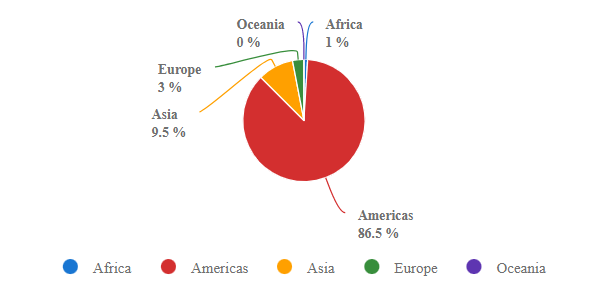
\includegraphics[width=12cm]{image/img1.png}
    \end{center}
    \legend{Fonte: \cite{FAOSTAT2022}}
\end{figure}


Neste mesmo período o Brasil deixou o posto de segundo lugar para ser o maior produtor de soja - na safra de 2001/2002, a produção brasileira era aproximadamente 52 milhões de toneladas, nesta mesma safra o EUA era aproximadamente 75 milhões de toneladas, agora na safra 2021/2022 o Brasil alcançou perto de 122 milhões toneladas, superior ao EUA que entorno de 120,7 milhões de toneladas, conforme dados da \cite{conab2022}.

\begin{figure}
  \caption{\label{imagen2}Produção de Soja por ano no Brasil de 1994 a 2020}
    \begin{center}
      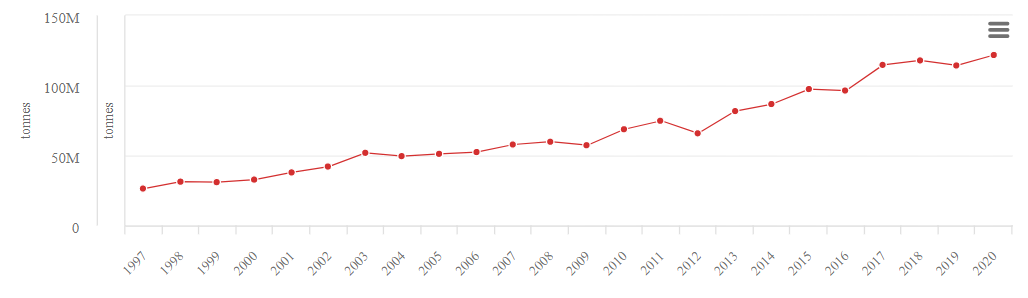
\includegraphics[scale = 0.7]{image/img2.png}
    \end{center}
    \legend{Fonte: \cite{FAOSTAT2022}}
\end{figure}


Diante do exposto deste trabalho, pretende à aplicação de modelos \textbf{ARIMA} (Autorregressivos Integrados de Médias Móveis) nos índices de preços da \textit{commodities} soja com a finalidade de compreender o comportamento da 
comercialização deste produto.


% ----------------------------------------------------------
% Capitulo de textual
% ----------------------------------------------------------
\chapter{Séries Temporais}
  
Qualquer conjunto de observações ordenadas no tempo, é uma série temporal. Por exemplos:

\begin{itemize}
  \item[\textit{i)}] temperaturas médias diárias de uma cidade;
  \item[\textit{ii)}] vendas mensais de uma empresa;
  \item[\textit{iii)}] valores de fechamento diários da IBOVESPA;
  \item[\textit{iv)}] preços diários de \textit{commodities};
  \item[\textit{v)}] valores mensais do IPCA (Índice Nacional de Preços ao Consumidor Amplo).
\end{itemize}

As séries temporais podem ser tanto discreta quanto contínua, ou seja, discreta é o 
intervalo entre as observações pertecentes a um conjunto discreto, e contínua é o 
intervalo entre as observações pertecentes a um conjunto contínuo. Observa-se que 
quando dizemos que uma série é discreta, estamos fazendo referência ao tempo entre as 
observações e não a escala da variável.

Além disso, temos dois enfoques usados na análise de séries temporais. O objetivo de ambos é construir modelos para as séries. No primeiro enfoque é feita análise no \textit{domínio temporal} e os modelos sugeridos são \textit{modelos paramétricos} (números de parâmetros finitos), o segundo é conduzido no \textit{domínio de frequências} e os propostos são 
\textit{modelos não-paramétricos} \cite{morettin2006analise}. O modelo utilizado neste 
estudo, \textbf{ARIMA} é um modelo paramétrico.




  \section{Processos Estocásticos}
  
Podemos definir um processo estocástico como um conjunto cronológico de observações de um determinado fenômeno de forma que o seu comportamento pode ser descrito por uma ou mais distribuições de probabilidade. Conforme \cite{morettin2006analise},


\begin{definition}

Seja $T$ um conjunto arbitrário, um processo estocástico é uma família de variáveis aleatórias 
$\left\{Z(t),\ t \in T \right\}$, tal que, $\forall t \in T$,  $Z(t)$ é uma variável aleatória.

\end{definition}
  
\begin{figure}
  \caption{\label{img4}Família de trajetórias de processos estocásticos.}
    \begin{center}
      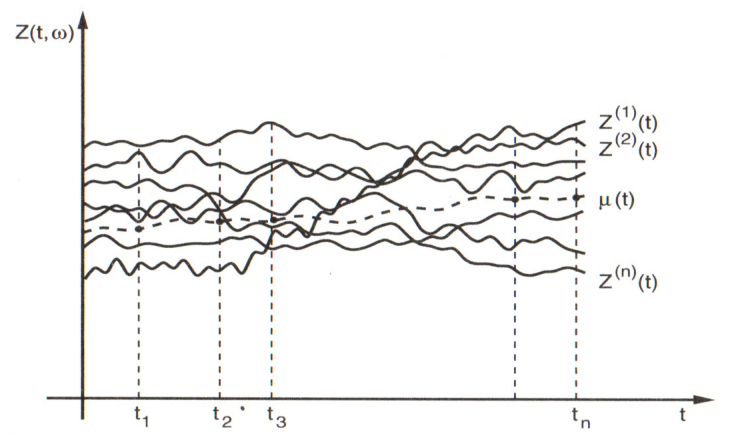
\includegraphics[scale = 0.9]{image/img4.png}
    \end{center}
    \legend{Fonte: \cite{morettin2006analise}}
\end{figure}

Neste caso, um processo estocástico é uma família de variáveis aleatórias, definidas num mesmo espaço de probabilidade $(\Omega, \mathcal{A}, \mathcal{P})$, tendo o conjunto $T$, normalmente tomado como conjunto dos inteiros $\mathbb{Z} = \left\{0,\pm 1, \pm 2, \ldots \right\}$ ou conjunto dos reais $\mathbb{R}$.

A Figura \ref{img3} ilustra uma interpretação de um processo estocástico, ou seja, para $t \in T,\ Z(t)$ é uma variável aleatória definida em $\Omega$, e $Z(t)$ é uma função de dois argumentos $Z(t, \omega)$, $t \in T$, $\omega \in \Omega$. Na figura, cada $t \in T$, temos uma v.a. $Z(t, \omega)$, com uma distribuição de probabilidade, é possível que a função densidade de probabilidade (fdp) no instante $t_1$ seja distinta da fdp no instante $t_2$, entre os instante $t_1$ e $t_2$ quaisquer, mas usualmente é aquela em que a fdp de $Z(t, \omega)$ é a mesma, $\forall t \in T$.



\begin{figure}
  \caption{\label{img3}Um processo estocástico interpretado como uma família de variáveis.}
    \begin{center}
      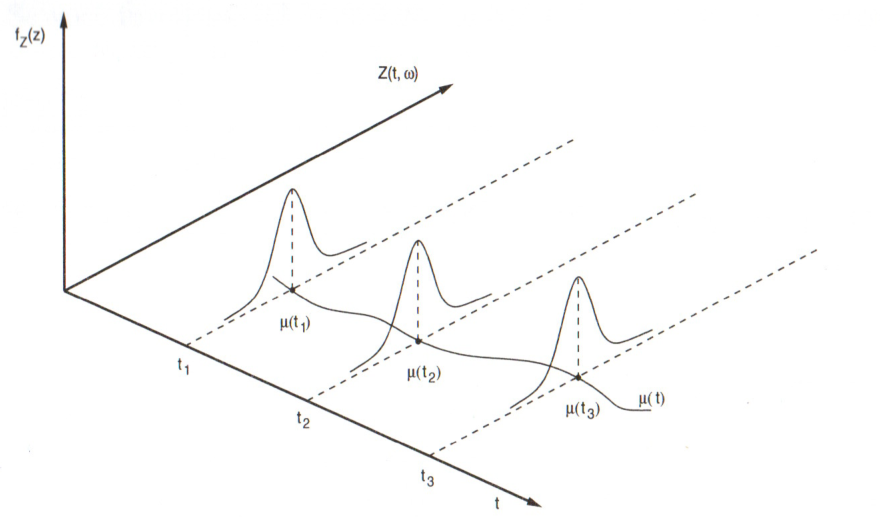
\includegraphics[scale = 0.9]{image/img3.png}
    \end{center}
    \legend{Fonte: \cite{morettin2006analise}}
\end{figure}




  \section{Processo Estocástico Estacionário}




  \section{Decomposição de um Série Temporal}
  
  
  
  
  
  \section{Modelos ARIMA}





\chapter{Metodologia}

Por 


Para obtenção das análises estatísticas dos dados, fez-se o uso do \textit{software} \textbf{R} versão 4.2.1


A 


O índice de Preços da \textit{commodities} Soja 



\chapter{Resultados e Discussões}




A Tabela \ref{tab1} apresenta as principais medidas descritivas obtidas a partir da série mensal 
condizente ao indicador de preços em reais da soja (reais por saca de 60 kg) compreendido 
no período de outubro de 1997 a outubro de 2022, proporcionanddo uma visão panorâmica do comportamento da série em estudo. 

\begin{knitrout}
\definecolor{shadecolor}{rgb}{0.969, 0.969, 0.969}\color{fgcolor}\begin{table}[!h]

\caption{\label{tab:script3}Estística Descritiva \label{tab1}}
\centering
\begin{tabular}[t]{rrrrrr}
\toprule
Min. & 1st Qu. & Median & Mean & 3rd Qu. & Max.\\
\midrule
\cellcolor{gray!6}{13.87} & \cellcolor{gray!6}{31.34} & \cellcolor{gray!6}{46.8} & \cellcolor{gray!6}{58.63} & \cellcolor{gray!6}{72.91} & \cellcolor{gray!6}{195.8}\\
\bottomrule
\end{tabular}
\end{table}

\end{knitrout}



A Figura \ref{fig1} apresenta a série original do indicador de preço em reais da soja no intervalo de outubro de 1997 a outubro de 2022 

\begin{knitrout}
\definecolor{shadecolor}{rgb}{0.969, 0.969, 0.969}\color{fgcolor}\begin{figure}[H]
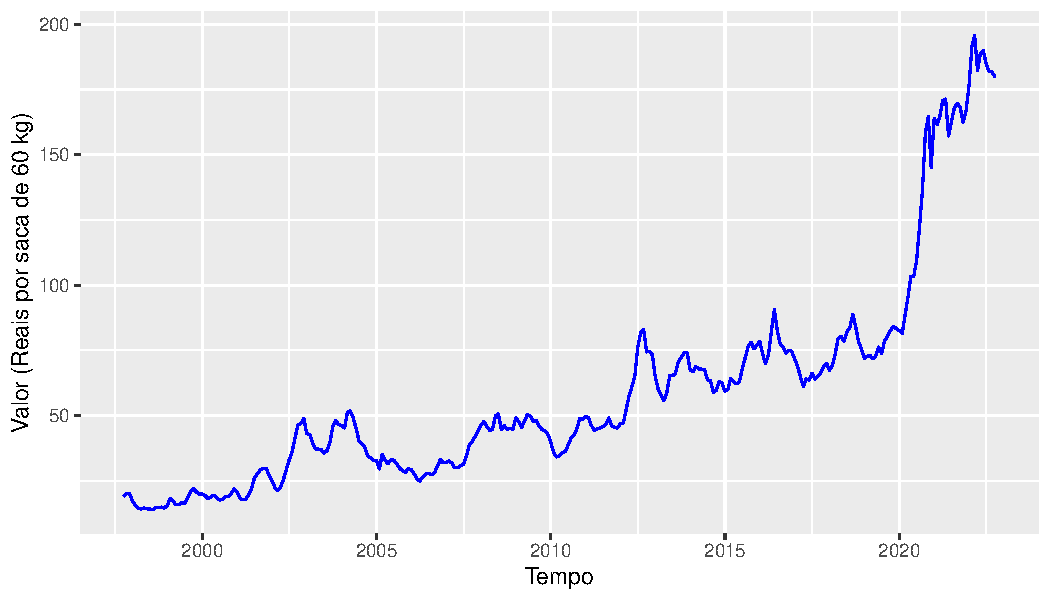
\includegraphics[width=\maxwidth]{figure/script1-1} \caption[Indicador de preço da soja no período de outubro de 1997 até outubro de 2022 \label{fig1}]{Indicador de preço da soja no período de outubro de 1997 até outubro de 2022 \label{fig1}}\label{fig:script1}
\end{figure}

\end{knitrout}




\begin{knitrout}
\definecolor{shadecolor}{rgb}{0.969, 0.969, 0.969}\color{fgcolor}\begin{figure}
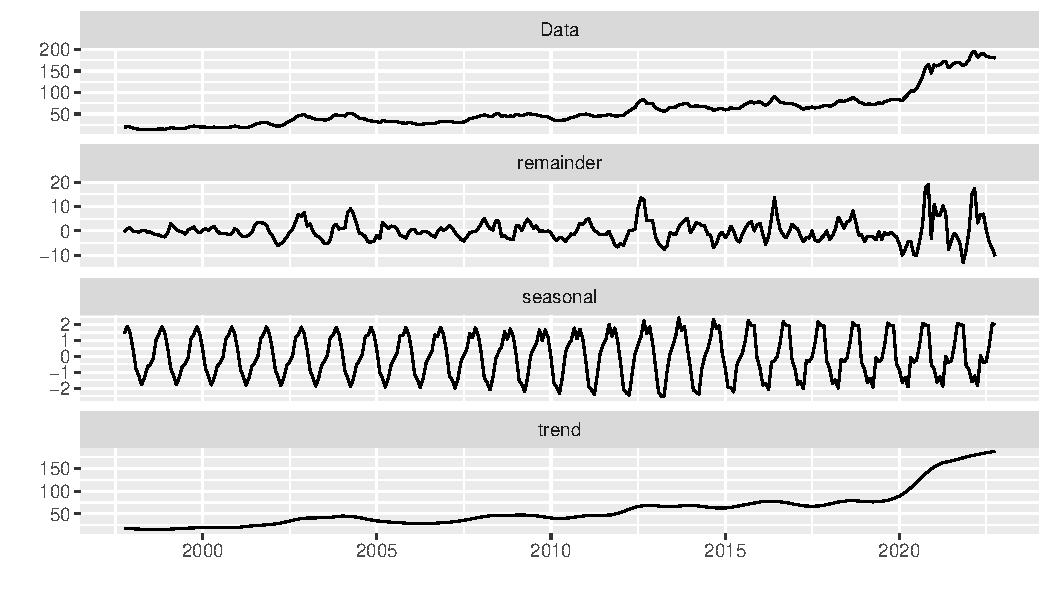
\includegraphics[width=\maxwidth]{figure/script2-1} \end{figure}

\end{knitrout}





\begin{knitrout}
\definecolor{shadecolor}{rgb}{0.969, 0.969, 0.969}\color{fgcolor}\begin{figure}
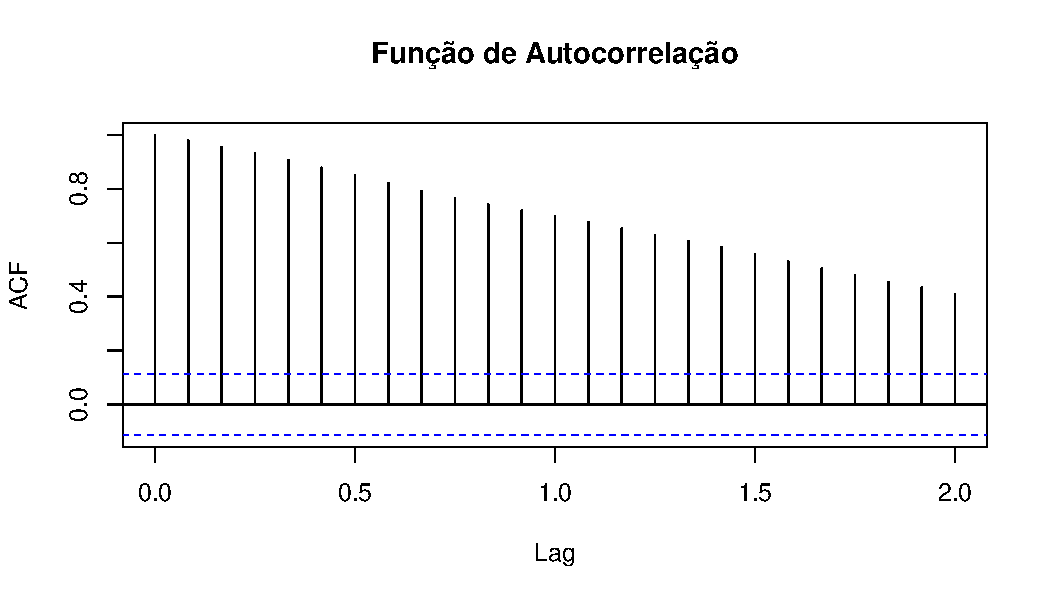
\includegraphics[width=\maxwidth]{figure/script4-1} \end{figure}

\end{knitrout}





\begin{knitrout}
\definecolor{shadecolor}{rgb}{0.969, 0.969, 0.969}\color{fgcolor}\begin{figure}
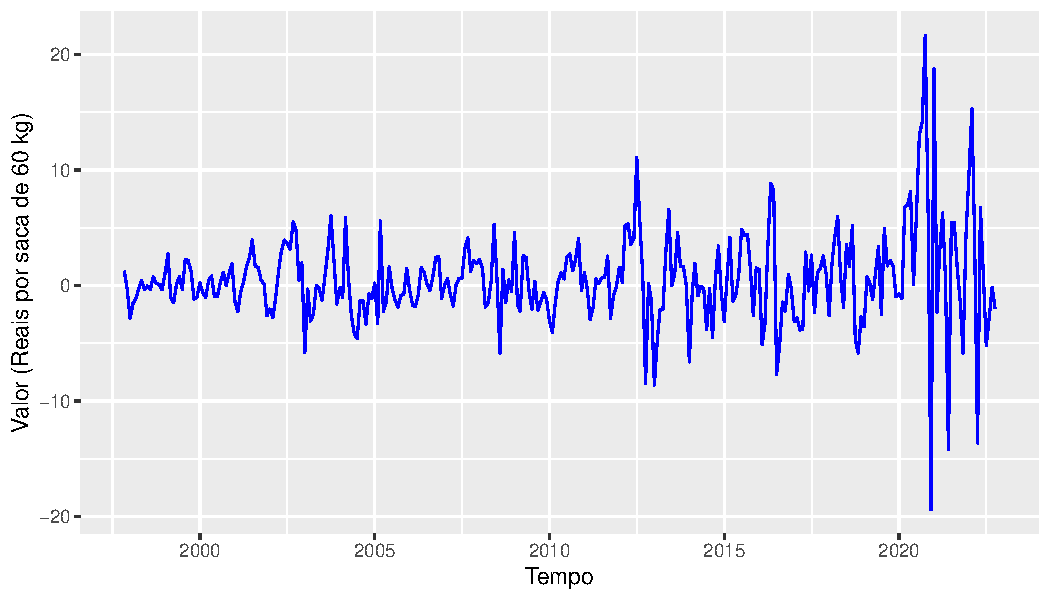
\includegraphics[width=\maxwidth]{figure/script5-1} \end{figure}

\end{knitrout}


\begin{knitrout}
\definecolor{shadecolor}{rgb}{0.969, 0.969, 0.969}\color{fgcolor}\begin{figure}
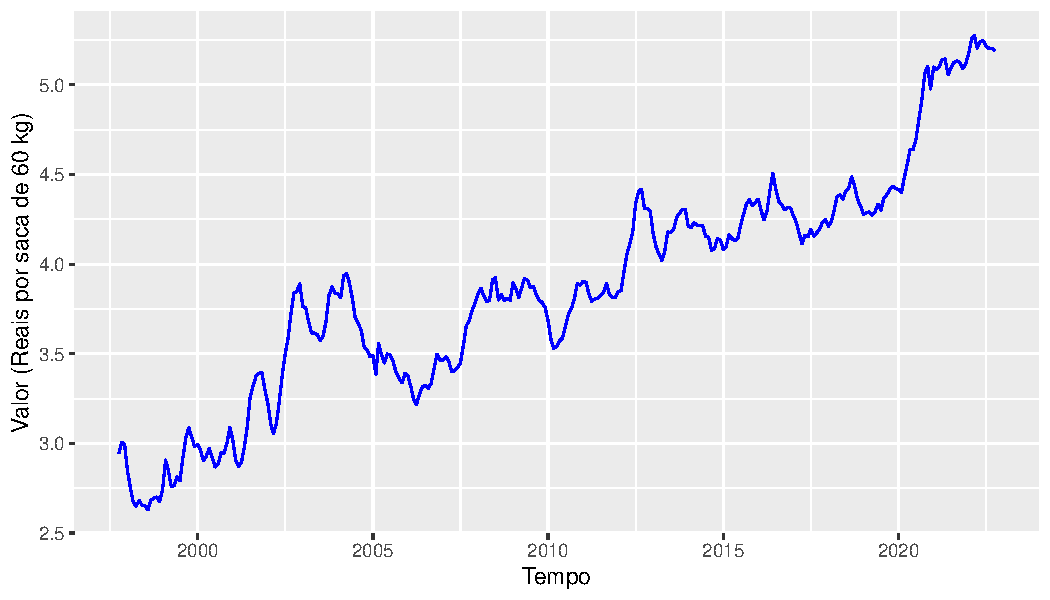
\includegraphics[width=\maxwidth]{figure/script6-1} \end{figure}

\end{knitrout}





\chapter{Considerações Finais}

O presente trabalho teve como objetivo estudar o comportamento do preço da Soja no Brasil, e testar a metodologia Box \& Jenkins para previsão.



% ----------------------------------------------------------
\bibliography{abntex2-modelo-references}

% ----------------------------------------------------------
% Glossário
% ----------------------------------------------------------
%
% Consulte o manual da classe abntex2 para orientações sobre o glossário.
%
%\glossary

% ----------------------------------------------------------
% Apêndices
% ----------------------------------------------------------

% ---
% Inicia os apêndices
% ---

% Tirar os restantes das páginas não textuais.



\begin{apendicesenv}

% Imprime uma página indicando o início dos apêndices
\partapendices

% ----------------------------------------------------------
\chapter{SCRIPT R}
% ----------------------------------------------------------

\begin{knitrout}\tiny
\definecolor{shadecolor}{rgb}{0.969, 0.969, 0.969}\color{fgcolor}\begin{kframe}
\begin{alltt}
\hlkwd{library}\hlstd{(forecast)}   \hlcom{# Ferramentas para exibir e analisar previsões de séries temporais univariadas.}
\hlkwd{library}\hlstd{(timeSeries)} \hlcom{# Ferramentas para séries temporais financeiras.}
\hlkwd{library}\hlstd{(urca)}       \hlcom{# Testes de raiz unitária e de cointegração.}
\hlkwd{library}\hlstd{(randtests)}  \hlcom{# Testes de aleatoriedade não paramétricos para sequências numéricas.}
\hlkwd{library}\hlstd{(tseries)}    \hlcom{# Análise de séries temporais e finanças computacionais.}
\hlkwd{library}\hlstd{(stats)}      \hlcom{# Funções para cálculos estatísticos e geração de números aleatórios.}
\hlkwd{library}\hlstd{(readxl)}     \hlcom{# Importe arquivos Excel para R.}
\hlkwd{library}\hlstd{(tidyverse)}  \hlcom{# Conjunto de pacotes que funcionam em harmonia para data analysis.}
\hlkwd{library}\hlstd{(ggfortify)}  \hlcom{# Ferramentas de plotagem unificadas.}
\hlkwd{library}\hlstd{(magrittr)}   \hlcom{# Fornece o encadeamento de comandos, pipeline (%>%).}
\hlkwd{library}\hlstd{(kableExtra)} \hlcom{# Gerador de tabelas.}

\hlstd{soja} \hlkwb{<-} \hlkwd{read_xls}\hlstd{(}\hlstr{"...dataset/soja.xls"}\hlstd{)} \hlcom{# Importar o conjunto de dados.}

\hlstd{soja} \hlkwb{<-} \hlkwd{ts}\hlstd{(soja}\hlopt{$}\hlstd{Preço,} \hlkwc{start} \hlstd{=} \hlkwd{c}\hlstd{(}\hlnum{1997}\hlstd{,}\hlnum{10}\hlstd{),} \hlkwc{frequency} \hlstd{=} \hlnum{12}\hlstd{)} \hlcom{# Criar o objeto de série temporal.}

\hlkwd{class}\hlstd{(soja)} \hlcom{# Retornar os valores do atributo de classe de um objeto.}
\hlkwd{as.ts}\hlstd{(soja)} \hlcom{# Testar se o objeto é um série temporal.}

\hlcom{### Informações descritiva da série (resumo).}
\hlkwd{summary}\hlstd{(soja)}

\hlcom{### Plotagem da série original.}
\hlkwd{autoplot}\hlstd{(soja,} \hlkwc{xlab} \hlstd{=} \hlstr{"Tempo"}\hlstd{,} \hlkwc{ylab} \hlstd{=} \hlstr{"Valor (Reais por saca de 60 kg)"}\hlstd{,} \hlkwc{ts.colour} \hlstd{=} \hlstr{'blue'}\hlstd{)}

\hlcom{### Decomposição da série e plotagem.}
\hlstd{soja} \hlopt
  \hlkwd{stl}\hlstd{(,} \hlkwc{s.window} \hlstd{=} \hlstr{"periodic"}\hlstd{)} \hlopt
    \hlkwd{autoplot}\hlstd{(,} \hlkwc{ts.colour} \hlstd{=} \hlstr{"blue"}\hlstd{)}

\hlcom{### }
\end{alltt}
\end{kframe}
\end{knitrout}





\end{apendicesenv}
% ---


\end{document}
